\documentclass[portuguese, a4paper]{article}
\usepackage[T1]{fontenc}
\usepackage[utf8]{inputenc}
\usepackage{babel}
\usepackage[margin=3cm]{geometry}
\usepackage{lmodern}

\usepackage{graphicx}
\graphicspath{ {imagens/} {flowcharts/}}
\usepackage{bold-extra}
\usepackage{epstopdf}
\usepackage{float}
\usepackage{scalerel}
\usepackage{enumerate}
\usepackage{indentfirst}
\usepackage{mathtools}
\usepackage{amsmath}
\allowdisplaybreaks
\usepackage{amssymb}
\usepackage{listings}
\usepackage{color}
\usepackage{textcomp}
\usepackage{caption}
\usepackage{hyperref}
\hypersetup{
    colorlinks,
    citecolor=black,
    filecolor=black,
    linkcolor=black,
    urlcolor=black
}

\newcommand\showdiv[1]{\overline{\smash{\hstretch{.5}{)}\mkern-3.2mu\hstretch{.5}{)}}#1}}
\newcommand\ph[1]{\textcolor{white}{#1}}
\newcommand\tu[0]{\textunderscore}

\definecolor{dkgreen}{rgb}{0,0.6,0}
\definecolor{gray}{rgb}{0.5,0.5,0.5}
\definecolor{mauve}{rgb}{0.58,0,0.82}
\definecolor{mygreen}{RGB}{28,172,0} % color values Red, Green, Blue
\definecolor{mylilas}{RGB}{170,55,241}

% ----- Cabeçalho e rodapé -----
\usepackage{fancyhdr}
\pagestyle{fancy}
\fancyhf{}

\renewcommand{\headrulewidth}{1pt}
\renewcommand{\footrulewidth}{0.5pt}

\rhead{Word Morph}
\lhead{Algoritmos e Estruturas de Dados}
\rfoot{Página \thepage}
\lfoot{\small Engenharia Eletrotécnica e de Computadores - IST}

\usepackage{pdfpages}

\begin{document}
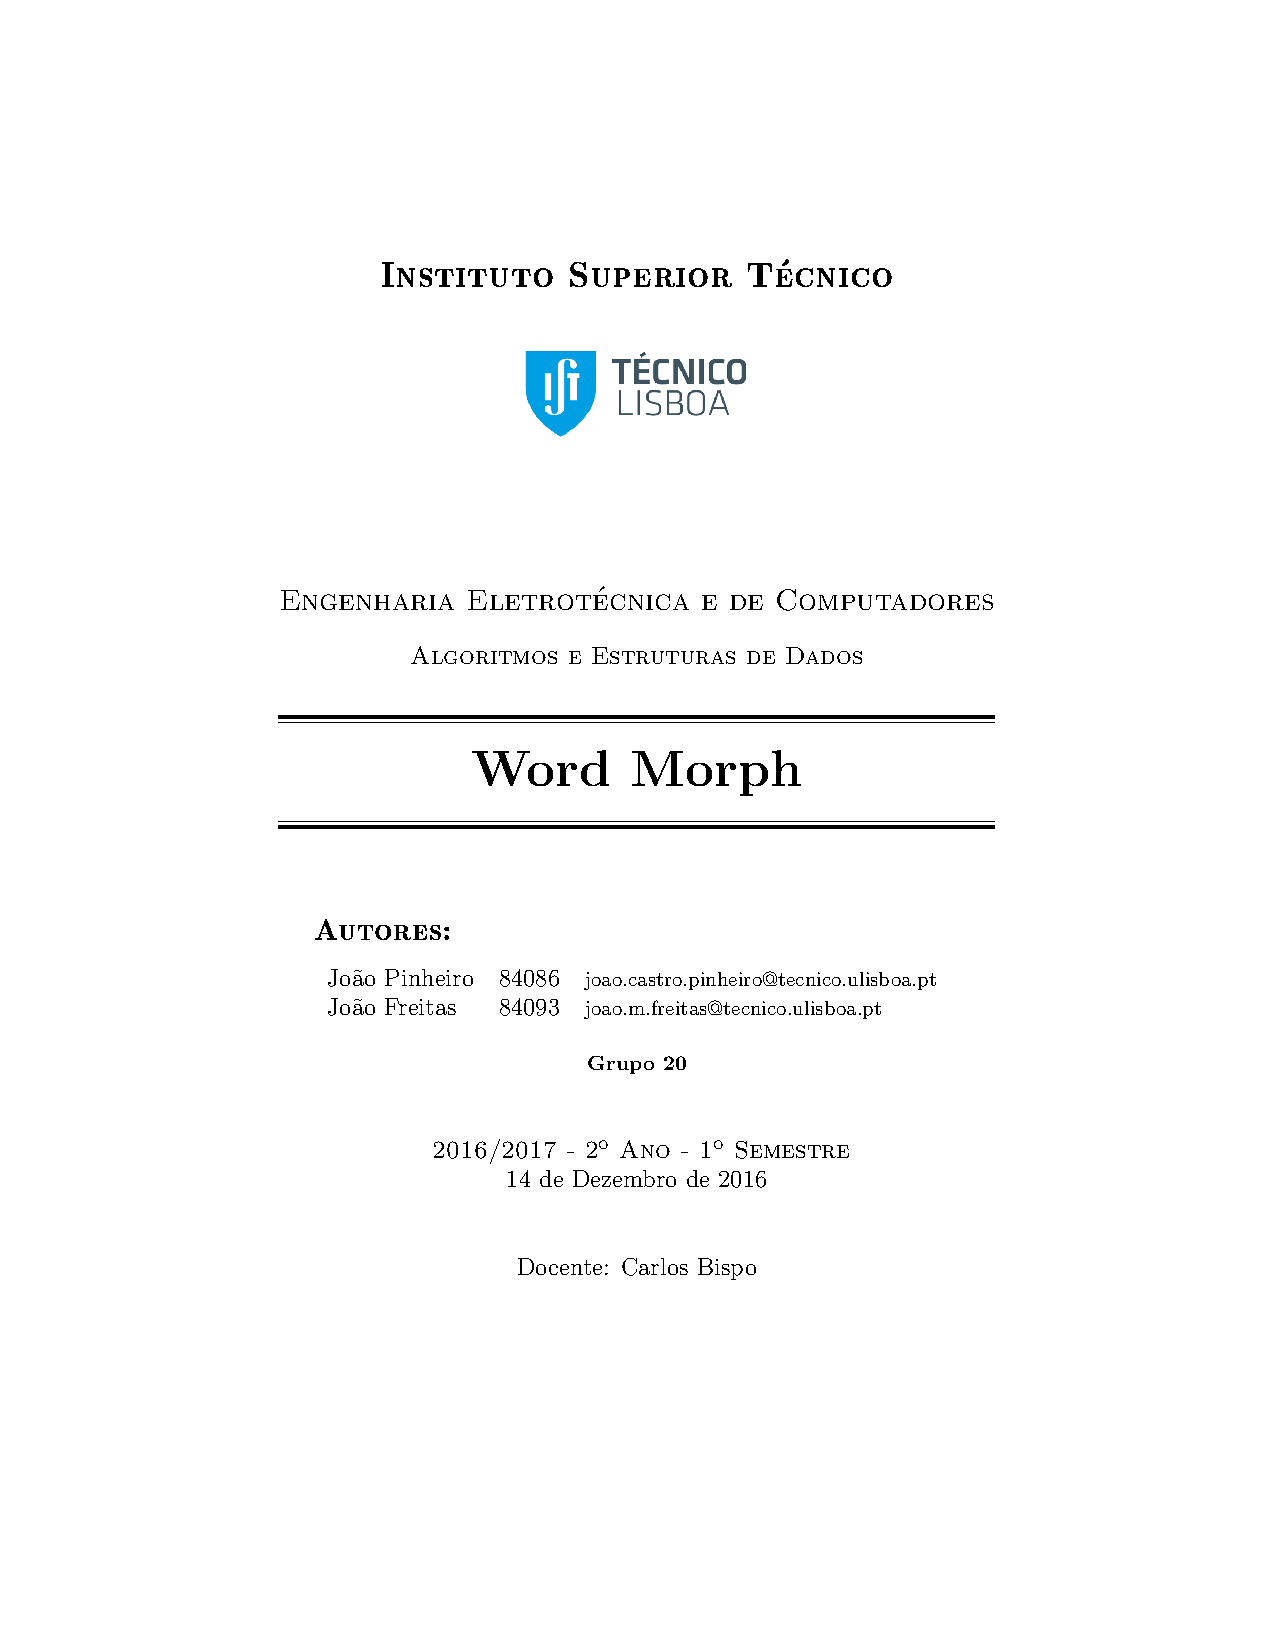
\includepdf[pages={1}]{capa/capa.pdf}

\tableofcontents
\newpage

\section{Especificação do problema}
	\par
	O problema proposto é encontrar caminhos entre duas palavras do mesmo
	tamanho. Estes caminhos consistem em permutações de letras. Em cada passo
	podem-se alterar no máximo um dado número de letras. No entanto, o peso duma
	ligação é o quadrado do número de carateres mudados. O objetivo é então
	encontrar o caminho de menor custo (i.e., que minimiza o peso total das
	ligações do caminho) entre a palavra de origem e a palavra de destino,
	passando por palavras do dicionário dado. Por exemplo, dado o problema:
	\begin{center}
		\texttt{dragar oravam 2}
	\end{center}
	\par
	É preciso encontrar o caminho de \textbf{dragar} a \textbf{oravam},
	permutando, no máximo, 2 palavras em cada passo. Um caminho válido é então:
	\begin{center}
		\textbf{dragar} \\
		tragam \\
		\textbf{oravam}
	\end{center}
	\par
	Através de duas mutações de dois carateres cada. O custo total deste caminho
	é $2 \times 2^2 = 8$. No entanto, um caminho de menor custo seria:
	\begin{center}
		\textbf{dragar} \\
		tragar \\
		tragam \\
		travam \\
		\textbf{oravam}
	\end{center}
	\par
	Através de 4 mutações de um carater cada. O custo total deste caminho é
	$4\times1^1 = 4$, sendo de menor custo do que o anterior e, deste modo, a
	resposta correta.
	\par
	Para resolver grandes quantidades destes problemas, implementou-se uma
	solução na linguagem \textit{C}. O programa recebe dois parâmetros: \\
	\begin{itemize}
		\item
		Um ficheiro de dicionário de extensão \texttt{.dic} de
		palavras não acentuadas, não hifenadas e não necessariamente ordenado
		alfabeticamente, no formato de palavras separadas por um só espaço e uma ou
		mais palavras por linha.
		\item
		Um ficheiro de problemas de extensão \texttt{.pal} com
		vários problemas, um por linha, no formato:
		\begin{center}
			\texttt{<origem> <destino> <número máximo de permutações>}
		\end{center}
		\par
		Onde se assume que o formato está correto e as palavras pertencem ao
		dicionário.
	\end{itemize}
	\par
	O programa é invocado então da seguinte maneira:
	\begin{center}
		\texttt{\$ ./wordmorph <dicionário.dic> <problemas.pal>}
	\end{center}
	\par
	O programa escreve um ficheiro de saída de extensão \texttt{.path},
	explicitando os caminhos e o custo associado, no seguinte formato, por
	exemplo, para o exemplo anterior \texttt{dragar oravam 2}:
	\begin{center}
		\texttt{
		dragar 4\\
		tragar \\
		tragam \\
		travam \\
		oravam}
	\end{center}
	\par
	É de notar que se não existir caminho, o peso será \texttt{-1}; se as
	palavras forem iguais, o peso será \texttt{0}. Existe uma linha em branco
	entre cada solução.


\section{Abordagem}
	\par
	Este problema é muito facilmente transposto num problema de grafos
	ponderados, em que os vértices representam palavras e as arestas ligações
	de $k$ permutações, sendo o peso da aresta igual a $k^2$.  Calcular os
	caminhos mais curtos entre palavras traduz-se então num problema de caminho
	mais curto fonte-destino em grafos, onde se conhecem algoritmos de boa
	complexidade tanto temporal como de memória.


\section{Arquitetura}
	\par
	O programa pode ser dividido abstratamente em 3 componentes lógicos:
	encontrar o numero maximo de permutações; construção do grafo; resolução dos
	problemas. Esta divisão logica está expressa nas funções
	\texttt{find\tu max\tu perm, read\tu dic, solve\tu pal} respectivamente.

	\par
	O fluxograma da figura \ref{geral} demonstra a organização do programa como
	explicada anteriormente.

	\begin{figure}[H]
		\centering
		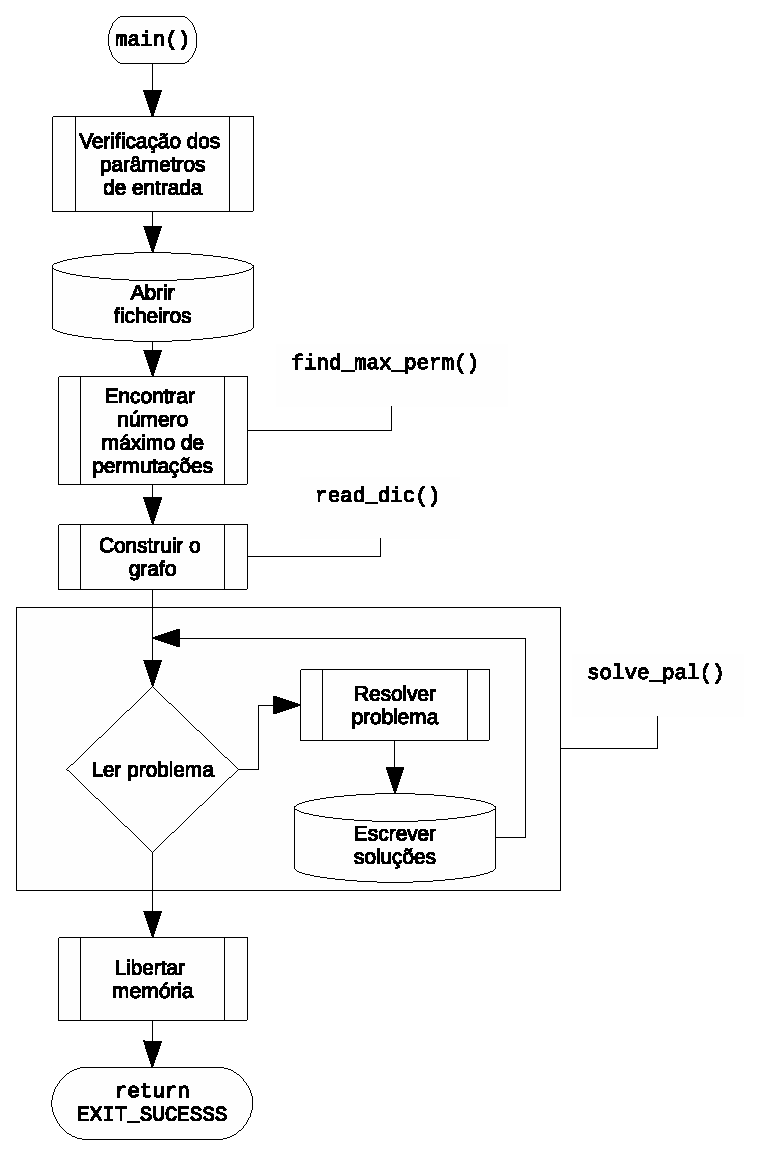
\includegraphics[width=0.70\linewidth]{main}
		\caption{Fluxograma principal do programa (função \texttt{main()}).}
		\label{geral}
	\end{figure}

	\par
	O fluxograma da figura \ref{make_graph} explicita a rotina \texttt{read\tu
	pal()}.
	\begin{figure}[H]
		\centering
		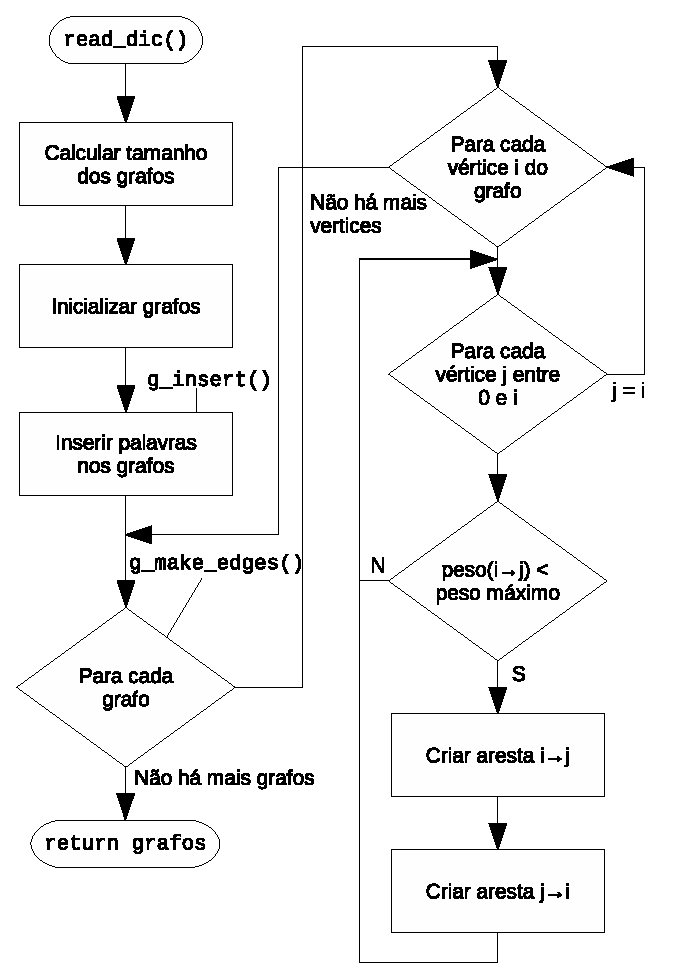
\includegraphics[width=0.70\linewidth]{read_dic}
		\caption{Fluxograma da função \texttt{read\tu dic()} que constrói o grafo.}
		\label{make_graph}
	\end{figure}
	\par
	O fluxograma figura \ref{solve_pal} sintetisa a rotina \texttt{solve\tu pal}.
	\begin{figure}[H]
		\centering
		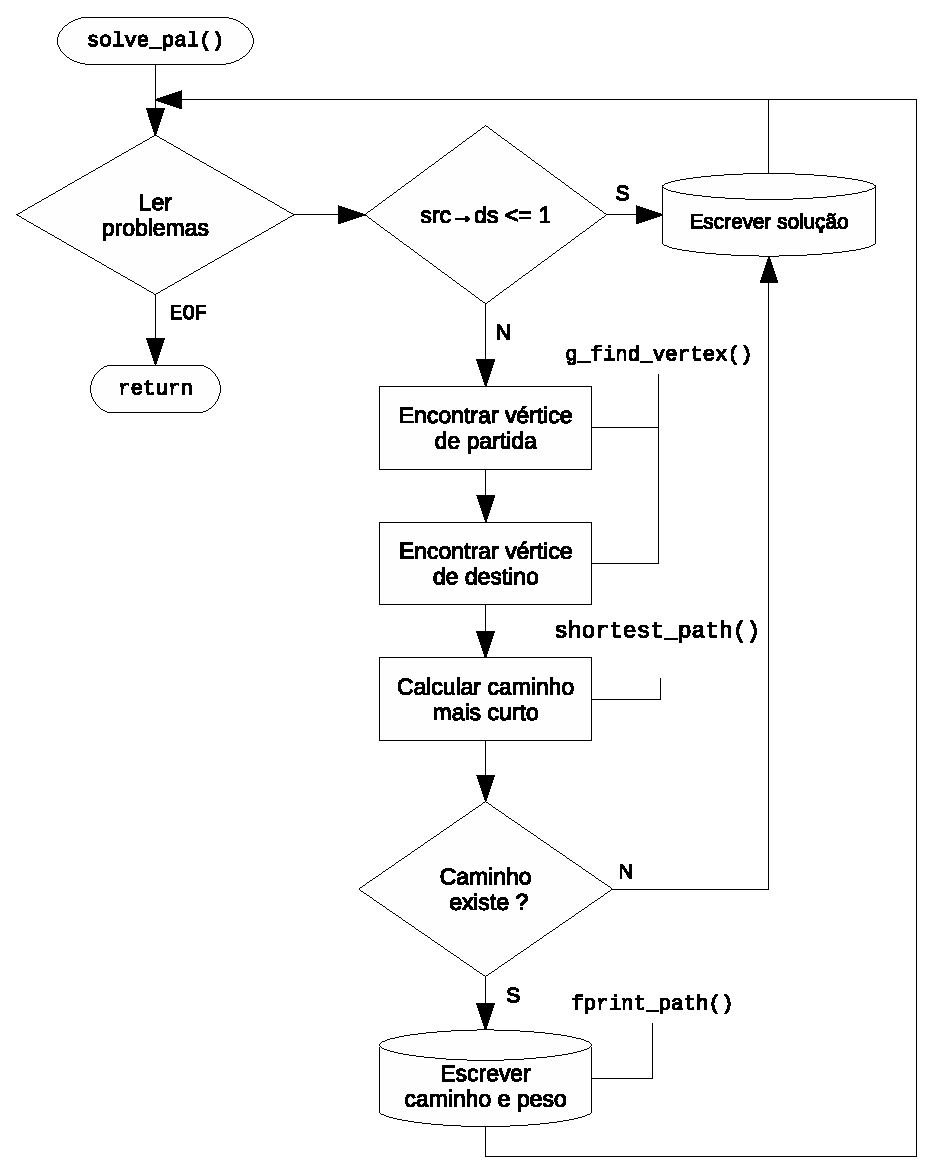
\includegraphics[width=0.70\linewidth]{solve_pal}
		\caption{Fluxograma da função \texttt{solve\tu pal()} que calcula e
		escreve os caminhos.}
		\label{solve_pal}
	\end{figure}
	\par
	A função \texttt{find\tu max\tu perms()} é detalhada na secção
	\ref{sec:alg}.
	\par
	As estruturas de dados, algoritmos e subsistemas utilizados no programa
	serão descritos mais aprofundadamente nas próximas secções.

\section{Estruturas de dados}
	\subsection{Grafo}
	\par
	Como podem existir vários tamanhos de palavras no ficheiro de problemas,
	pode ser necessário construir mais do que um grafo. Decidiu-se utilizar uma
	tabela de grafos indexada por um inteiro representando o tamanho de palavras
	que um grafo contém. Optou-se por representar o grafo por listas de
	adjacências por estes se provarem ser relativamente esparsos, poupando assim
	memória face à implementação através de matriz de adjacências. Os elementos
	mais relevantes da estrutura \texttt{Graph} são a tabela de vértices, o
	número de vértices e o peso máximo das arestas do grafo.
	\par
	Um vértice contém um tipo de dados genérico (neste caso, as palavras do
	dicionário) e também um ponteiro para a cabeça duma lista ''implícita''
	\footnote{explicação na secção \ref{sec:analise}.}, simplesmente ligada, de
	arestas para os vértices adjacentes.
	\par
	Por sua vez, uma aresta contém o índice do vértice a que liga, o peso da
	ligação e um ponteiro para a próxima aresta da lista dum vértice
	particular.

	\subsection{Acervo}
	\par\null\par
	A outra estrutura de dados relevante é o acervo, utilizado como fila
	prioritária no cálculo dos caminhos mais curtos, devido às suas operações
	assimtoticamente eficientes. A implementação é sob a forma de tabela de tipo
	de dados genérico, que identifica um vértice.
	\par
	O acervo contém ainda uma tabela de dispersão simples, que efetua o
	mapeamento contrário à tabela de elementos do acervo (i.e., é indexada pelo
	item identificador de um vértice e guarda a posição deste na tabela de
	elementos do acervo), permitindo assim procura em tempo constante na
	estrutura. Assim, utiliza-se o índice inteiro do vértice no grafo e a função
	de dispersão torna-se trivial e assegura que não haverá colisões.

	\begin{figure}[H]
		\centering
		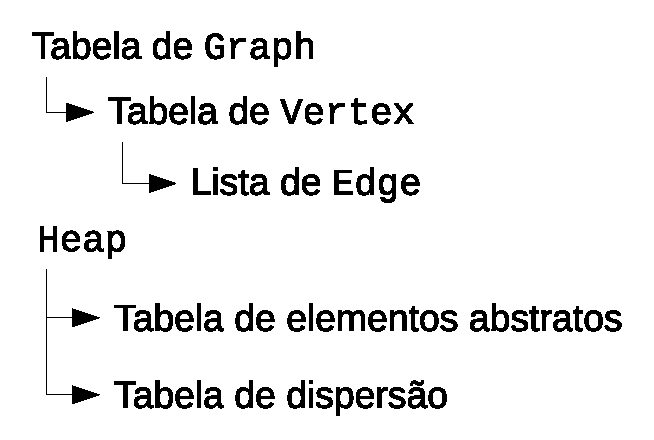
\includegraphics[width=0.4\linewidth]{data}
		\caption{Diagrama das principais estruturas de dados utilizadas.}
	\end{figure}


\section{Algoritmos}
\label{sec:alg}
	\par
	Devido às restrições de tempo e memoria impostas foi
	necessário utilizar algoritmos que pudessem ser executados em tempo útil e
	que fizessem uma gestão eficiente da memória.

	\subsection{Calcúlo do numero máximo de permutações}
	\par
	\texttt{}
	\subsection{Grafo}
	\subsubsection{Criação de arestas}
	\par
	Após a leitura das palavras e da inserção dos vértices no grafo é necessário
	criar as arestas entre os vértices. O algoritmo responsável pela execução
	da tarefa é um dos mais simples e inefecientes neste projecto. Segue-se uma
	descrição simples do algoritmo, implementado na função \texttt{g\tu make\tu
	edges()}.

	\par\null\par
	\texttt{Para cada vértice i do grafo}\\
	\indent\indent\texttt{Para cada vértice j de 0 até i}\\
	\indent\indent\indent\texttt{Criar aresta i->j}\\
	\indent\indent\indent\texttt{Criar aresta j->i}\\

	\par
	Como o grafo é não direcionado é possével criar ao mesmo tempo a aresta
	entre vértice i e o vértice j e a ligação entre o vértice j e o vértice i.
	\subsubsection{Procura}
	\par
	O algoritmo de procura utilizado é a simples procura linear, implementado
	na funcao \texttt{g\tu find\tu vertex()}. Poderia ter sido implementado,
	por exemplo, o algoritmo de procura binária, mas tal implicaria ordenar
	alfabeticamente o grafo. Verificou-se também que a procura linear não
	afetava substancialmente o tempo de execução do programa. Assim, por estas
	duas razões, decidiu-se não aumentar a complexidade do programa
	implementando um algoritmo de ordenação eficiente e a procura binária.

	\subsection{Acervo}
	\par
	A eficiência do algoritmo de Dijkstra depende muito da eficiência das
	operações da estrutura de dados utilizada como fila prioritária.
	\par
	Devido à forma natural dos acervos, em arvore binária balançada de
	prioridades, remover o elemento mais prioritário é uma operação trivial,
	assim como as operações de inserção, fixup e fixdown.
	% TODO: melhor explicação do fixup e fixdown?
	\par
	Por outro lado, a procura por um elemento no acervo permanece linear uma
	vez que não existe nenhum critério óbvio de divisão do problema. Por esse
	motivo foi implementada uma tabela de dispersão que permite o
	mapeamento entre um elemento e a sua posição no acervo.  Esta alteração
	permite saber atualizar a prioridade de um elemento da heap em tempo
	logarítmico, eliminando um factor linear devido à procura.

	\subsection{Algoritmo de Dijkstra}
	\label{sec:alg_dijkstra}
	\begin{figure}[H]
		\centering
		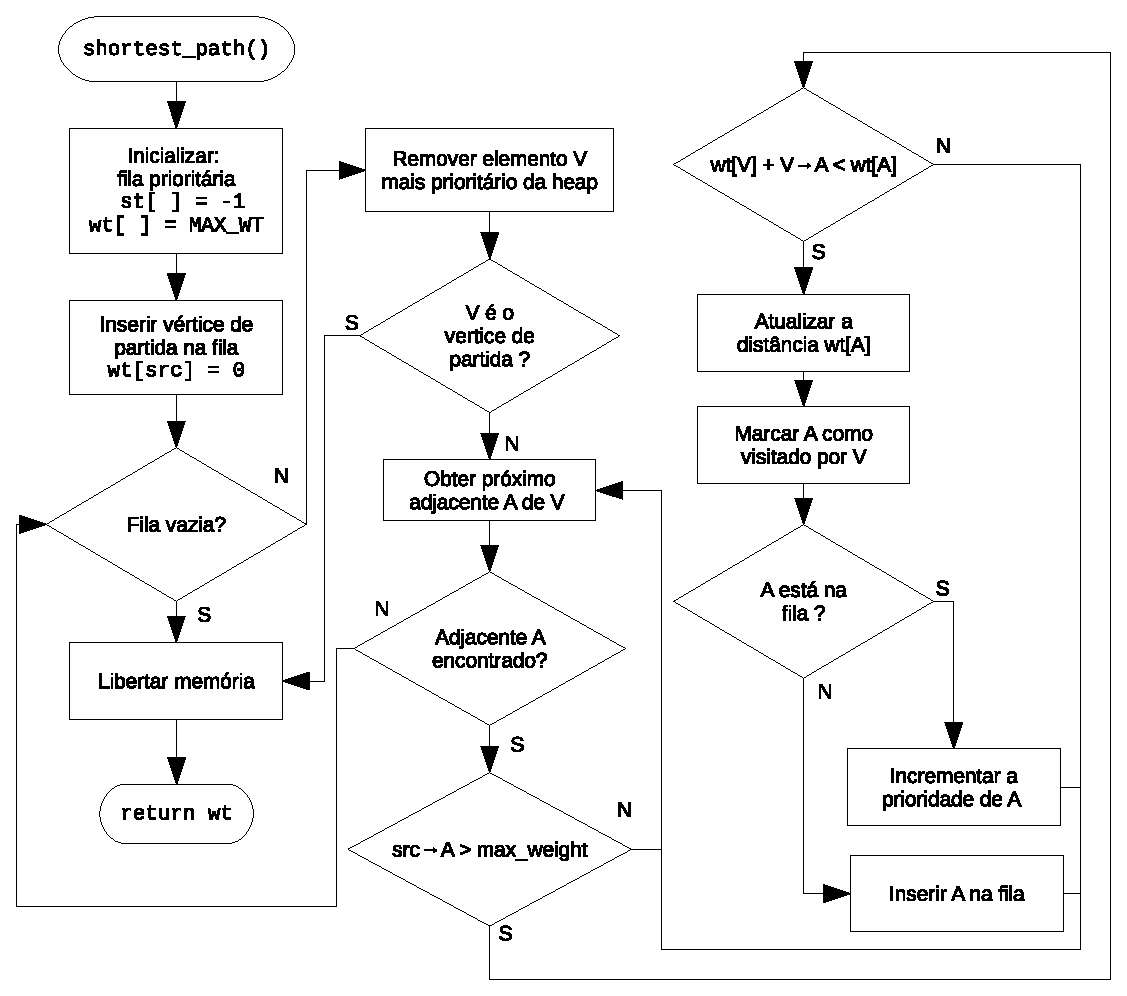
\includegraphics[width=0.85\linewidth]{dijkstra}
		\caption{Fluxograma da implementação do algoritmo de Dijkstra.}
		\label{fig:dijkstra}
	\end{figure}
	\par
	Para o cálculo de caminhos mais curtos entre palavras foi implementado uma
	versão ligeiramente modificada do algoritmo de Dijkstra, descrita no
	fluxograma da figura \ref{fig:dijkstra}.
	\par
	Na sua forma original o algoritmo de Dijkstra calcula caminhos estre um
	vértice e todos os outros vértices do grafo. Como tal não é necessário,
	nesta implementação paramos a execução do algoritmo assim que o vértice de
	destino sai da fila prioritária.
	\par
	Do mesmo modo, a operação de colocar todos os vértices do grafo na fila
	prioritária é extremamente ineficiente devido ao elevado número de
	vértices mas também por processar vértices para os quais nem existe caminho
	a partir do vértice de partida. Em alternativa basta colocar inicialmente
	apenas o vértice de partida na fila, processá-lo e em seguida colocar os
	seus adjacentes na fila.

	\subsection{Impressão de caminho}
	\par
	O algoritmo de Dijkstra devolve uma árvore de caminhos mais curtos entre os
	vértices do grafo\footnote{Alguns caminhos estarão incompletos devido a
	optimizações descritas na secção \ref{sec:alg_dijkstra}. De qualquer forma o
	caminho entre os vértices de partida e de chegada estará completo.} e o vértice
	de partida. Para imprimir esse caminho é necessário percorrê-lo em ordem
	inversa.
	\par
	A resolução do problema torna-se simples utilizando uma função
	recursiva que percorre o caminho do fim para o início e imprime os vértices
	assim que a função retorna, utilizando assim a stack implicíta que é criada
	na invocação de funções.


\section{Análise de complexidade}
	\par
	A complexidade das funções de leitura e escrita de ficheiros, do subsistema \texttt{file.c}, têm todas complexidade $O(n)$, devido à sua natureza de acesso ao disco.

	\subsection{Grafo}
	\par
	A complexidade em termos de memória do programa é majorada na prática pela
	memória ocupada pelos grafos. Esta é proporcional a $O(V + E)$ em que $V$ é
	o número de vértices e $E$ o número de arestas.

	\subsubsection{Criação de arestas}
	\par
	Os ciclos \texttt{for} da função \texttt{g\tu make\ edges()} têm
	complexidade $O(\frac{1}{2}V^2) = O(V^2)$. Contando com a função de
	comparação de caracteres das palavras, seria necessário multiplicar por um
	outro fator que representa o tamanho das palavras.

	\subsubsection{Procura}
	\par
	Como referido na secção \ref{sec:alg}, a procura no grafo é linear, de
	complexidade $O(V)$.

	\subsection{Acervo}
	\par
	A operação de inserção no acervo é de tempo constante $O(1)$ pois este é
	implementado com uma tabela. Pela estrutura natural do acervo, as operações
	\texttt{h\tu fixup()} e \texttt{h\tu fixdown()} são, no pior caso, de
	complexidade $O(lg~n)$, em que $n$ é o número de elementos na heap.
	\par
	A procura no acervo tem complexidade $O(1)$, com recurso a uma tabela de
	dispersão. Assim, a função \texttt{h\tu inc\tu pri()} tem complexidade
	$O(1) + O(lg~n) = O(lg~n)$.

	\subsection{Algoritmo de Dijkstra}
	\par
	O algoritmo de Dijkstra pode ser separado em duas partes lógicas,
	inicializações e o loop principal. As inicializações têm complexidade $O(V)
	+ O(1) = O(V)$.  Dentro do ciclo \texttt{while} principal, no pior caso o
	caminho percorre todos os vértices da fila, e assim a função \texttt{del\tu
	max\tu pri}, de complexidade $O(lg~V)$, é chamada $V$ vezes. Para cada
	aresta, terá de incrementar a sua prioridade, com complexidade de $2E *
	O(lg~V)$, em que $E$ é o número de arestas. Assim, a complexidade total é:
	\cite{randompdf}
	$$O(V) + VO(lg~V) + 2E~O(lg~V) = O((V + E)lg~V)$$

	\subsection{Impressão de caminho}
	\par
	Esta função tem complexidade $O(n)$, proporcional ao número de vértices $n$
	no caminho.


\section{Subsistemas}
	\subsection{file}
	\begin{itemize}
		\item \textbf{Objetivos}
		\par
		Agrupa as funções que lidam com escrita e leitura de ficheiros.

		\item \textbf{Módulos}
		\par
		\texttt{file.c} e \texttt{file.h}

		\item \textbf{Funções}
		\par
		\texttt{unsigned short *find\tu max\tu perms(FILE *fpal)}
		\par
		Devolve uma tabela com o número máximo de permutações, por tamanho de
		palavras, vindo do ficheiro .pal.

		\par\null\par
		\texttt{Graph **read\tu dic(FILE *fdic, unsigned short *max\tu perms)}
		\par
		Devolve uma tabela de grafos cujos índices são tamanhos de palavras e
		os vértices palavras do dicionário.

		\par\null\par
		\texttt{void solve\tu pal(FILE *fpal, FILE *fpath, Graph **graphs)}
		\par
		Encontra e escreve no ficheiro de sáida .path as soluções aos
		problemas.

		\par\null\par
		\texttt{void fprint\tu path(FILE *fpath, Graph *g, int *st, int *wt,
		int dst)}
		\par
		Escreve o caminho do vértice de origem até ao vértice de destino
		\texttt{dst} pela ordem correta, a partir da árvore de caminhos
		\texttt{st}.
	\end{itemize}

	\subsection{word}
	\begin{itemize}
		\item \textbf{Objetivos}
		\par
		Implementa o tipo de dado principal do programa (\texttt{char *}),
		utilizado como Item dos vértices.

		\item \textbf{Módulos}
		\par
		\texttt{word.c} e \texttt{word.h}

		\item \textbf{Funções}
		\par
		\texttt{Item w\tu new(char *word)}
		\par
		Aloca e devolve uma nova palavra, a utilizar como tipo de dados
		genérico \texttt{Item}.

		\par\null\par
		\texttt{void w\tu free(Item word)}
		\par
		Liberta uma palavra.

		\par\null\par
		\texttt{unsigned short w\tu diff(Item v1, Item v2, unsigned short
		max\tu perm)}
		\par
		Devolve o número de caracteres diferentes, até a \texttt{max\tu perm},
		entre duas palavras de tamanhos iguais.

		\par\null\par
		\texttt{int w\tu cmp(Item v1, Item v2)}
		\par
		Compara duas palavras utilizando \texttt{strcmp()} e devolve o mesmo
		valor que esta função.
	\end{itemize}

	\subsection{graph}
	\begin{itemize}
		\item \textbf{Objetivos}
		\par
		Implementa as estruturas de dados Grafo, Vértice e Aresta.

		\item \textbf{Módulos}
		\par
		\texttt{graph.c} e \texttt{graph.h}

		\item \textbf{Funções}
		\par
		\texttt{Graph *g\tu init(unsigned short size, unsigned short max\tu
		weight)}
		\par
		Aloca e devolve um grafo.

		\par\null\par
		\texttt{void g\tu free(Graph *g, void (free\tu item)(Item item))}
		\par
		Liberta um grafo.

		\par\null\par
		\texttt{void g\tu insert(Graph *g, Item i)}
		\par
		Insere o Item \texttt{i} na posição livre do grafo.

		\par\null\par
		\texttt{void g\tu make\tu edges(Graph *g, unsigned short (*calc\tu weight)(Item
				i1, Item i2, unsigned short max))}
		\par
		Cria arestas entre os vértices se quaisquer dois diferirem no máximo de
		\texttt{max} caracteres.

		\par\null\par
		\texttt{unsigned short g\tu get\tu size(Graph *g)}
		\par
		Função acessora do número máximo de vértices no grafo.

		\par\null\par
		\texttt{unsigned short g\tu get\tu free(Graph *g)}
		\par
		Função acessora da posição livre do grafo.

		\par\null\par
		\texttt{unsigned short g\tu get\tu max\tu weight(Graph *g)}
		\par
		Função acessora do peso máximo das arestas do graof.

		\par\null\par
		\texttt{Vertex *g\tu get\tu vertex(Graph *g, unsigned short i)}
		\par
		Função acessora de um vértice \texttt{i} do grafo.

		\par\null\par
		\texttt{int g\tu find\tu vertex(Graph *g, Item i1, int (*cmp\tu item)(Item c1,
		Item c2))}
		\par
		Encontra um vértice \texttt{i1} no grafo.

		\par\null\par
		\texttt{Vertex *v\tu init(Item i)}
		\par
		Aloca e devolve um vértice.

		\par\null\par
		\texttt{Item v\tu get\tu item(Vertex *v)}
		\par
		Função acessora ao tipo de dados genérico de um vértice \texttt{v}.

		\par\null\par
		\texttt{Edge *v\tu get\tu adj(Vertex *v)}
		\par
		Função acessora ao ponteiro para a cabeça da lista de adjacências de um
		vértice \texttt{v}.

		\par\null\par
		\texttt{void e\tu add(Graph *g, unsigned short i1, unsigned short i2, unsigned
				short weight)}
		\par
		Adiciona duas arestas: do vértice \texttt{i1} ao vértice \texttt{i2} e
		vice-versa com peso \texttt{weight}.

		\par\null\par
		\texttt{unsigned short e\tu get\tu weight(Edge *e)}
		\par
		Função acessora ao peso duma aresta \texttt{e}.

		\par\null\par
		\texttt{unsigned short e\tu get\tu index(Edge *e)}
		\par
		Função acessora ao índice do vértice ao qual a aresta \texttt{e} liga.

		\par\null\par
		\texttt{void free\tu adj(Edge *head)}
		\par
		Liberta a lista de adjacências de um vértice através do ponteiro para a
		cabeça da lista.

		\par\null\par
		\texttt{void e\tu insert(Edge **adj, unsigned short index, unsigned short
				weight)}
		\par
		Cria uma aresta até ao vértice de índice \texttt{index} com peso
		\texttt{weight} na lista de adjacências \texttt{adj} de um vértice.

		\par\null\par
		\texttt{Edge *e\tu get\tu next(Edge *l)}
		\par
		Função acessora à aresta a seguir da aresta \texttt{l} na lista de
		adjacências de um vértice.
	\end{itemize}

	\subsection{dijkstra}
	\begin{itemize}
		\item \textbf{Objetivos}
		\par
		Implementa a função \texttt{shortest\tu path()} para encontrar caminhos
		mais curtos entre vértices do grafo.

		\item \textbf{Módulos}
		\par
		\texttt{dijkstra.c} e \texttt{dijkstra.h}

		\item \textbf{Funções}
		\par
		\texttt{int *shortest\tu path(Graph *g, int src, int dst, int *st,
		unsigned short max\tu weight)}
		Encontra o caminho mais curto entre os vértices \texttt{src} e
		\texttt{dst} no grafo \texttt{g}. Escreve o caminho na árvore de
		caminhos \texttt{st} e devolve a tabela de distâncias.

		\par\null\par
		\texttt{bool d\tu less\tu pri(Item s1, Item s2)}
		\par
		Função de comparação de prioridade utilizada pelo acervo. Devolve
		\texttt{true} se \texttt{s1} tiver menos prioridade que \texttt{s2} ou
		falso se tiver maior ou igual.

		\par\null\par
		\texttt{unsigned short d\tu hash(Item a)}
		\par
		Função de dispersão utilizada pelo acervo. Devolve o índice no grafo do
		Item \texttt{a}.
	\end{itemize}

	\subsection{heap}
	\begin{itemize}
		\item \textbf{Objetivos}
		\par
		Implementação da estrutura de dados Acervo a utilizar como fila
		prioritária na função \texttt{shortest\tu path()}.

		\item \textbf{Módulos}
		\par
		\texttt{heap.c} e \texttt{heap.h}

		\item \textbf{Funções}
		\par
		\texttt{Heap *h\tu init(unsigned short size)}
		\par
		Aloca e devolve um novo acervo.

		\par\null\par
		\texttt{void h\tu free(Heap *h)}
		\par
		Liberta um acervo.

		\par\null\par
		\texttt{void h\tu fixup(Heap *h, int i, bool (*less\tu pri)(Item, Item), \\
		unsigned short (*hash)(Item))}
		\par
		Move um elemento do acervo para cima até à sua nova posição, de forma a
		manter a condição de acervo.

		\par\null\par
		\texttt{void h\tu fixdown(Heap *h, int i, bool (*less\tu pri)(Item, Item), \\
		unsigned short (*hash)(Item))}
		\par
		Move um elemento do acervo para baixo até à sua nova posição, de forma a
		manter a condição de acervo.

		\par\null\par
		\texttt{void h\tu insert(Heap *h, Item a, bool (*less\tu pri)(Item, Item), \\
		unsigned short (*hash)(Item))}
		\par
		Insere o Item \texttt{a} no acervo.

		\par\null\par
		\texttt{Item h\tu del\tu max\tu pri(Heap *h, bool (*less\tu pri)(Item, Item), \\
		unsigned short (*hash)(Item))}
		\par
		Devolve e remove o elemento de maior prioridade no acervo.

		\par\null\par
		\texttt{unsigned short h\tu find(Heap *h, Item a, unsigned short(*hash)(Item))}
		\par
		Devolve o índice de um Item \texttt{a} no acervo.

		\par\null\par
		\texttt{void h\tu inc\tu pri(Heap *h, Item a, bool (*less\tu pri)(Item, Item), \\
		unsigned short (*hash)(Item))}
		\par
		Move um elemento do acervo, que teve a sua prioridade aumentada, para
		cima até à sua nova posição, de forma a manter a condição de acervo.

		\par\null\par
		\texttt{void h\tu exch(Heap *h, unsigned short i1, unsigned short i2, \\
		unsigned short (*hash)(Item))}
		\par
		Troca dois elementos no acervo.

		\par\null\par
		\texttt{bool h\tu empty(Heap *h)}
		\par
		Devolve \texttt{true} se o acervo estiver vazio, \texttt{false} se não.
	\end{itemize}


\section{Análise crítica}
\label{sec:analise}
	\par
	Inicialmente, foram implementadas listas simplesmente ligadas de tipo de
	dados abstrato, num módulo separado, para o efeito das listas de adjacências
	dos vértices. No entanto, nestas condições verificou-se uma utilização
	excessiva de memória, muito superior ao valor esperado para os testes
	oferecidos pelo corpo docente. Decidiu-se então utilizar uma solução com
	listas ''implícitas'', i.e., com um ponteiro para a cabeça da lista
	(ponteiro para aresta) dentro da estrutura do vértice e um poteiro para a
	próxima aresta dentro da estrtura da aresta em si. No entanto, foram ainda
	implementadas funções acessoras a esta lista, por necessidade.
	\par
	Deste modo, verificou-se que a utilização de memória caiu para tanto quanto
	a metade na maioria dos testes. Tal explica-se pelo facto de a implementação
	por tipo de dados abstrato utilizar mais ponteiros, e, assim, mais memória,
	duma maneira muito percétivel, devido ao elevado número de arestas criadas
	durante a execução do programa.
	\par\null\par
	Existirão porventura algumas otimizações não implementadas, como uma
	procura mais eficiente no grafo, ou otimizações para lidar com casos mais
	extremos dos ficheiros de entrada, por exemplo, para lidar com números
	máximos de permutações muito grandes vindos do ficheiro de problemas. No
	entanto, este facto não se revelou um problema nos testes e, no caso geral,
	o programa comporta-se assintoticamente bem.


\section{Exemplo de execução}
	\par
	Por exemplo, para o ficheiro de problemas:
	\begin{center}
		\texttt{tragar travam 2}
	\end{center}
	\par
	E para o dicionário:
	\begin{center}
		\texttt{tragar tragam travam a flores}
	\end{center}
	\par
	Depois de verificar os parâmetros de entrada e abrir os ficheiros,
	\texttt{find\tu max\tu perms()} é chamada.  Inicializa \texttt{max\tu perms}
	a zero e de seguida o ficheiro de problemas é lido: como \texttt{w\tu
	diff()} devolve 2 e \texttt{max\tu perms[6] = 0 < 2}, então \texttt{max\tu
	perms[6] = 2} e os valores nos restantes índices ficam iguais a zero.
	\par
	A seguir constrói-se o grafo, chamando \texttt{read\tu dic()}. Esta função
	primeiramente lê o dicionário à procura do número de palavras de cada
	tamanho a alocar e chega apenas a \texttt{num\tu words[6] = 4}, ignorando a
	palavra de tamanho 1  pois \texttt{max\tu perms[1] = 0}. Seguidamente,
	\texttt{graphs[6]} é inicializado com 4 vértices (palavras), ficando os
	restantes valores nos índices \texttt{i} de \texttt{graphs} iguais a
	\texttt{NULL} pois representam os restantes tamanhos de palavra em que
	\texttt{max\tu perms = 0}. Agora o dicionário é lido outra vez para alocar
	as palavras em si, sendo \texttt{g\tu insert()} e \texttt{w\tu new()}
	chamadas 4 vezes, correspondendo às 4 palavras de tamanho 6. A seguir é
	chamada \texttt{g\tu make\tu edges()} para construir as arestas entre os
	vértices do grafo de tamanho de palavra 6. A tabela de vértices é:
	\texttt{[0: "tragar", 1: "tragam", 2: "travam", 3: "flores"]}.
	\par
	Os resultados dos ciclos em \texttt{g\tu make\tu edges()} são apresentados
	de seguida:
	\begin{itemize}
		\item
			\texttt{i = 0, j = 0} \\
			\texttt{---------------------}
		\item
			\texttt{i = 1, j = 0} \\
			\texttt{calc\tu weight("tragam", "tragar", 2) = 1} \\
			\texttt{e\tu add(g, 1 ("tragam"), 0 ("tragar"), 1)}
		\item
			\texttt{i = 2, j = 0} \\
			\texttt{calc\tu weight("travam", "tragar", 2) = 2} \\
			\texttt{e\tu add(g, 2 ("travam"), 0 ("tragar"), 4)}
		\item
			\texttt{i = 2, j = 1} \\
			\texttt{calc\tu weight("travam", "tragam", 2) = 1} \\
			\texttt{e\tu add(g, 2 ("travam"), 1 ("tragam"), 1)}
		\item
			\texttt{i = 3, j = 0} \\
			\texttt{calc\tu weight("flores", "tragar", 2) = 3}
		\item
			\texttt{i = 3, j = 1} \\
			\texttt{calc\tu weight("flores", "tragam", 2) = 3}
		\item
			\texttt{i = 3, j = 2} \\
			\texttt{calc\tu weight("flores", "travam", 2) = 3}
	\end{itemize}
	\par
	O grafo resultante como representado no programa, sob listas de adjacências
	(à direita) e graficamente (à esquerda) é: \\
	\begin{minipage}{\linewidth}
		\centering
		\begin{minipage}{0.45\linewidth}
		\begin{center}
			\texttt{0: 1 \textrightarrow{} 2 \textrightarrow{} NULL \\
					1: 0 \textrightarrow{} 2 \textrightarrow{} NULL \\
					2: 0 \textrightarrow{} 1 \textrightarrow{} NULL \\
					3: NULL}
		\end{center}
		\end{minipage}
		\hspace{0.05\linewidth}
		\begin{minipage}{0.45\linewidth}
			\begin{figure}[H]
				\centering
				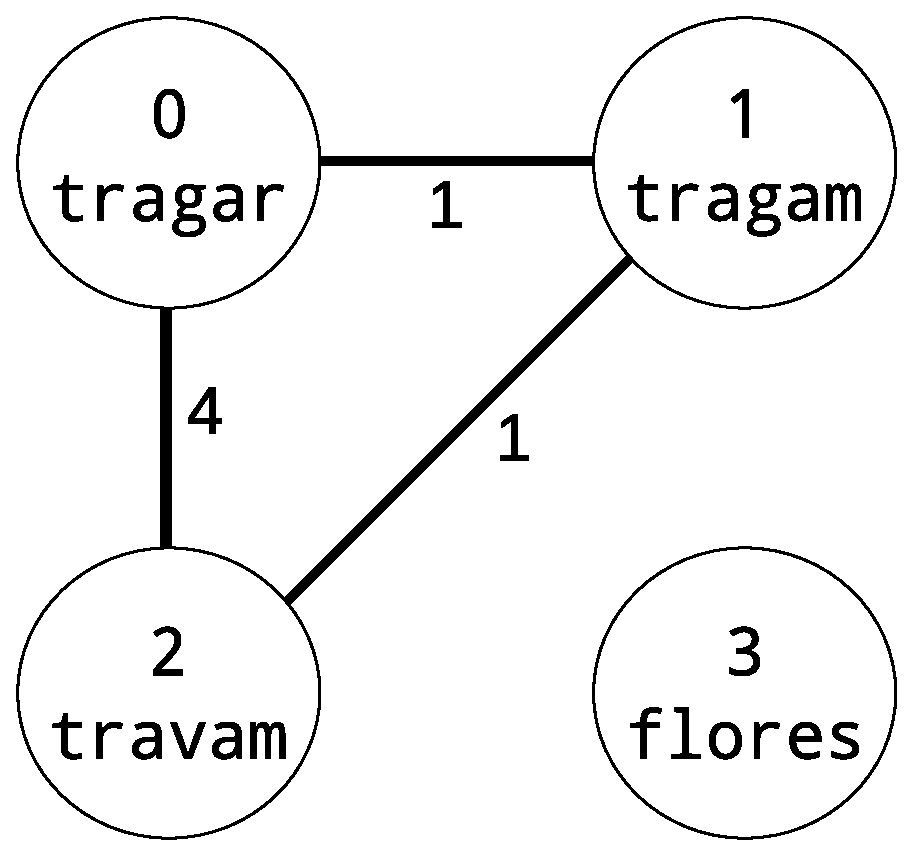
\includegraphics[width=4cm]{graph}
				\caption{Representação gráfica do grafo de exemplo}
			\end{figure}
		\end{minipage}
	\end{minipage} \\
	\par
	Construído o grafo, salta-se para a função \texttt{solve\tu pal()}.  O
	ficheiro de problemas é lido outra vez. Como \texttt{w\tu diff("tragar",
	"travam", 1) = 2 > 1}, a solução não é trivial. Deste modo, encontramos o
	vértice de origem, correspondente a \texttt{"tragar"} e o de destino
	\texttt{"travam"}, (re)aloca-se a árvore de caminhos \texttt{path} e
	corre-se \texttt{shortest\tu path()}.
	\par
	Esta função primeiramente inicializa um acervo, (re)aloca a tabela de
	distâcias à origem \texttt{wt} e inicializa-a com o valor \texttt{MAX\tu
	WT} representando uma distância infinita e inicializa a árvore de caminhos
	\texttt{st} com \texttt{-1} sinalizando que nenhum vértice foi visitado. O
	vértice de origem é também inserido no acervo inicialmente e a sua
	distância à origem é colocada a \texttt{0}. Apresenta-se o estado final das
	sucessivas iterações do ciclo \texttt{while} exterior do algoritmo de
	Dijkstra: \footnote{Os 'x' na tabela de dispersão do acervo representam
	índices ainda não utilizados ou que já não pertencem ao acervo, mas, na
	verdade, no programa, serão ou zero (inicializado com \texttt{calloc()}) ou
	o valor que lá estava da última vez que foi utlizado, que pode ou não ainda
	apontar para um elemento válido no acervo.}
	\begin{center}
		\begin{minipage}{0.45\linewidth}
		\texttt{\\
		v = 0\\
		v != dst (= 2) \\
		wt = [0, 1, 4, MAX\tu WT] \\
		st = [-1, 0, 0, -1] \\
		heap->vector = [1, 2] \\
		heap->hash\tu table = [x, 0, 1, x] \\}
		\end{minipage}
	\end{center}
	\par
	Na primeira iteração, o vértice \texttt{0} saiu da fila e foram colocados os
	seus adjacentes \texttt{1} e \texttt{2}, tendo sido marcados como visitados
	por \texttt{0} em \texttt{st} e com distâncias, respetivamente, \texttt{1} e
	\texttt{4} em \texttt{wt}. O acervo ficou com o vértice \texttt{1} na
	posição 0 mais prioritária então por este ter menor distância e assim maior
	prioridade. Assim, o vértice 1 sairá do acervo na próxima iteração:
	\begin{center}
		\begin{minipage}{0.45\linewidth}
			\texttt{\\
			v = 1\\
			v != dst (= 2) \\
			wt = [0, 1, 2, MAX\tu WT] \\
			st = [-1, 0, 1, -1] \\
			heap->vector = [2] \\
			heap->hash\tu table = [x, x, 0, x] \\}
		\end{minipage}
		\hspace{0.05\linewidth}
	\end{center}
	\par
	Os vértices adjacentes de 1 são \texttt{0} e \texttt{2}, mas \texttt{0} não
	entrará no acevo pois a sua distância (\texttt{0}) já é menor do que vista
	pelo vértice \texttt{1} (\texttt{1}). O vértice \texttt{2} tem a sua
	prioridade incrementada, pois, a partir do vértice \texttt{1}, a sua
	distância à origem é \texttt{wt[1] + 1 = 1 + 1 = 2} que é menor que a
	previamente encontrada de \texttt{wt[2] = 4}. Assim, o vértice 2 passa a
	ocupar a posição mais prioritária no acervo e sairá deste na próxima
	iteração:
	\begin{center}
		\begin{minipage}{0.45\linewidth}
		\texttt{\\
			v = 2 \\
			v == dst \\
			wt = [0, 1, 2, MAX\tu WT] \\
			st = [-1, 0, 1, -1] \\
			heap->vector = [2] \\
			heap->hash\tu table = [x, x, 0, x] \\}
		\end{minipage}
		\hspace{0.05\linewidth}
	\end{center}
	\par
	O vértice de destino saiu do acervo e parou-se a procura. A execução
	regressa a \texttt{solve\tu pal()} que escreverá o peso \texttt{wt[dst] = 2}
	e o caminho para este problema:
	\begin{center}
	\begin{minipage}{0.15\linewidth}
		\texttt{tragar 2 \\
				tragam \\
				travam}
	\end{minipage}
	\end{center}
	\par
	Onde o caminho foi impresso na ordem correta pela função recursiva
	\texttt{fprint\tu path()} (seguindo o caminho para trás desde
	\texttt{st[dst]} até chegar ao ponto inicial onde \texttt{st[src] = -1}).

\section{Bibliografia}
	\begin{thebibliography}{9}
		\bibitem{randompdf}
		K. Mehlhorn e P. Sanders, ''Shortest Paths,'' in
		\href{http://people.mpi-inf.mpg.de/~mehlhorn/ftp/Toolbox/ShortestPaths.pdf}{\emph{Algorithms
		and Data Structures: The Basic Toolbox}}. Berlim, Alemanha: Springer,
		2008, cap. 10, sec. 4, pp. 199.

		\bibitem{livro1}
		R. Sedgewick, \emph{Algorithms in C, Parts 1-4}, 3a edição. Boston:
		Addison Wesley, 1997.

		\bibitem{livro2}
		R. Sedgewick, \emph{Algorithms in C, Part 5}, 3a edição. Boston:
		Addison Wesley, 1997.
	\end{thebibliography}
\end{document}
